\chapter{Na-22 measurement}

In a PET system the excitation energy of the incident $\gamma$ is 511 KeV. As stated previously, at this energy a series of different processes intervene and contribute to the time resolution measured.
Three elements should be considered, when comparing time profiles to those measured with VUV radiation:
\begin{itemize}
\item production of Cerenkov photons
\item volume excitation (and so transit time spread in the bulk)
\item de excitation down to the thermalization region
\end{itemize}
The relative strengths of these phenomena have already been compared in chapter 6, and the possibility of measuring at high energy allows to physically quantify these effects.
In particular a time correlated single photon counting (TCSPC) system based on a $^{22}$Na source has been implemented, using a tagging crystal and a SiPM as a start signal and a MCP-PMT as a stop signal. The commissioning of this system is the object of this chapter and preliminary results are presented in comparison with VUV excitation.

\section{Phenomenology}

The physics of $\gamma$ photon interaction have been already introduced in chapter 2.
In order to build a time correlated single photon counting experiment two time signals are necessary, a start signal and a stop signal.
A simple way to obtain this is to use a $\beta ^{+}$ active isotope, such as $^{22}$Na. 
It emits a positron according to the decay reaction $^{22}Na \rightarrow ^{22}Ne + \beta ^{+} + \nu _{e} + \gamma$. The positron yield is relatively high, $90.4\%$, and competitive processes are electron capture (EC) and direct transition to the Ne ground state. 
In the positron emission case the Ne ground state is reached after 3.7 ps by emission of a $\gamma$ quantum of 1.274 MeV, as shown in figure \ref{fig:Na_22}. The half life of the isotope is 2.6 years.
\begin{figure}[htbp]
\begin{center}
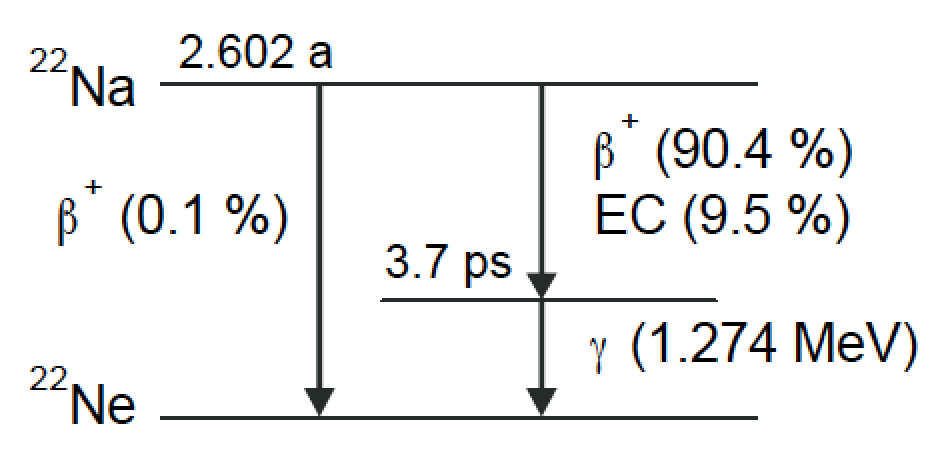
\includegraphics[width=8cm]{../Pictures/Chapter_8/Na-22}
\end{center}
\caption[Na$^{22}$ decay scheme]{Decay scheme of Na$^{22}$}
\label{fig:Na_22}
\end{figure}
It is worth to note that, as outlined in chapter 2 the Cerenkov threshold for heavy scintillators is below the energy of the annihilation $\gamma$ produced by the isotope.

\section{Experimental setup}

\begin{figure}[htbp]
\begin{center}
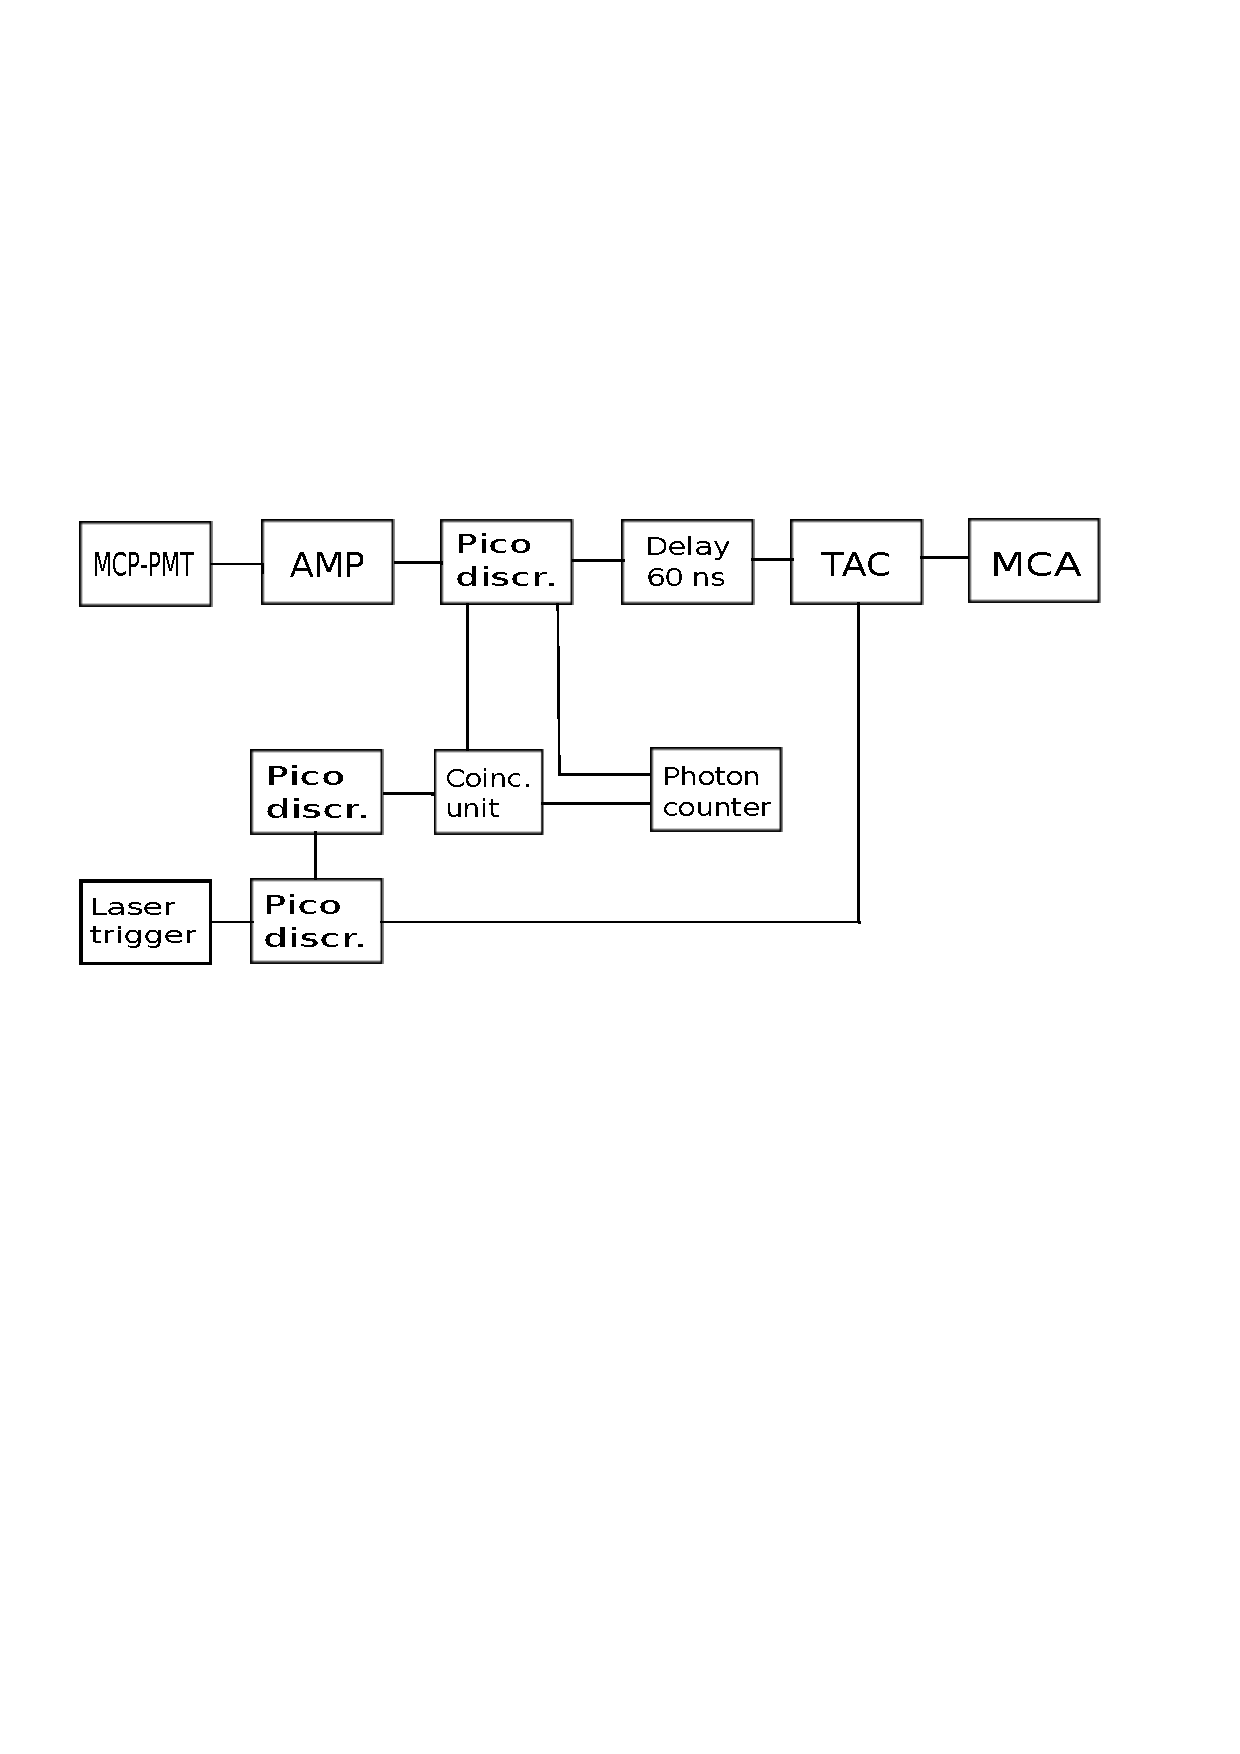
\includegraphics[width=6cm]{../Pictures/Chapter_8/electronics.pdf}
%qui una bella foto?
%\includegraphics[width=8cm]{../Pictures/Chapter_8/electronics.png}
\end{center}
\caption[Setup for $\gamma$ measurement]{The setup and DAQ for the $\gamma$ measurement is shown.}
\label{fig:setup}
\end{figure}
The scheme of the setup is shown in figure \ref{fig:setup}.
The tagging crystal used in this configuration is a 2x2x5 mm$^{3}$ LSO:Ce,Ca pixel, readout by a SiPM board amplified by a NINO chip. 
% glue? cerca misure del mppc!
The SiPM mounted on the board is a 3x3 mm$^{2}$ Hamamatsu MPPC S10931-050P with 50 $\mu$m cell size.
Its signal is then fed into the NINO chip described in chapter 3. The NINO technology, thanks to the time-over-threshold technique, collects time and energy information at the same time, thus allowing for a complete cut analysis.
The SiPM was biased through the board at 72.5 V, and the NINO at the nominal working voltage of 2.5 V. Moreover a potentiometer installed in the board allows to set up the lower and higher threshold for the NINO chip, as will be discussed in the following paragraph.
The signal is directly coupled to a high-bandwidth oscilloscope, able to digitize the pulses, a LeCroy DDA 735Zi (10 GS/s).
A sample of the NINO signal is shown in figure \ref{fig:NINO_sign}.
\begin{figure}[htbp]
\begin{center}
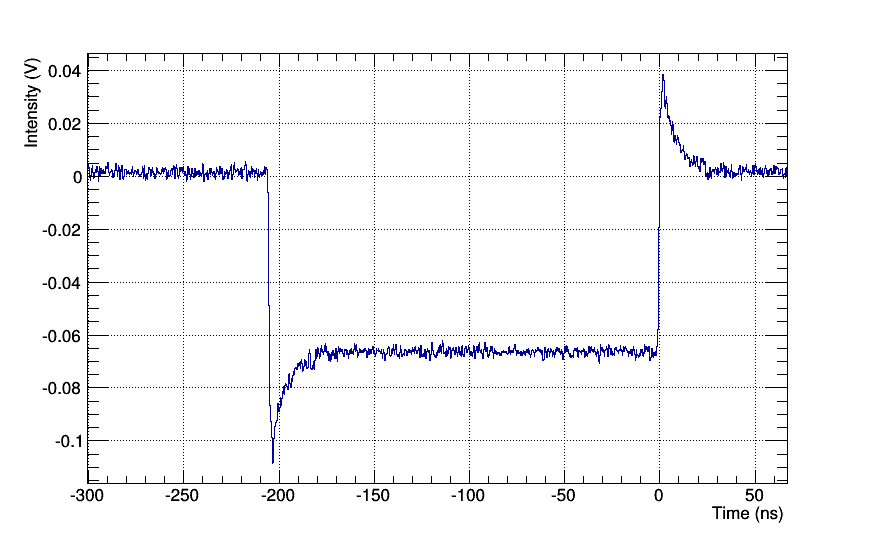
\includegraphics[width=10cm]{../Pictures/Chapter_8/NINO_signal.png}
\end{center}
\caption[NINO signal sample]{Example of NINO output from SiPM signal.}
\label{fig:NINO_sign}
\end{figure}
The stop signal is directly routed into the oscilloscope without amplification. The stop detector is a Hamamatsu R3809U-50 MCP-PMT.
The signal of the MCP is very fast, as can be seen in figure \ref{fig:MCP_sign}, since it is almost completely contained in 1 ns. This allows for a multi photon detection setup.
Indeed the two signal lines from the oscilloscope were saved for off line analysis, acting as a completely digitalization of the signal.
\begin{figure}[htbp]
\begin{center}
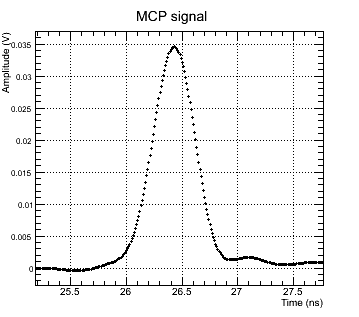
\includegraphics[width=8cm]{../Pictures/Chapter_8/MCP_signal.png}
\end{center}
\caption[MCP signal sample]{Example of Hamamatsu MCP-PMT output.}
\label{fig:MCP_sign}
\end{figure}
The components of the apparatus were placed in a cooled light-tight box, and the temperature held at 20 $\pm 1$ $^{\circ}$C degree tolerance.
Cooling is necessary to maintain stable the performance of SiPM. Indeed the number of thermal electrons that give rise to dark counts in the detector is strongly dependant on the temperature.
In the setup presented, as already pointed out, the accumulation times can be quite slow. It is necessary to keep the number of detected photon low, so that no significant bias is introduced in the measurement. The number of starts is thus much bigger than the number of stop at the acquisition. In order to gather data for a reasonable accumulation time, it is essential to reduce to the minimum the time the acquisition system (i.e. the oscilloscope) is busy.
The MCP benefits from temperature stability as well, and for the same reasons, but the noise level is negligible if compared to the SiPM.
Moreover the threshold set for the SiPM plays an important role on the DCR level of the device: in this case the DCR at 200 mV threshold is 0.88 Mcps (for complete discussion see \cite{Gundacker2014}). 

% cita gundi e piazza il valore
%spiegare e mostrare il setup della board cioe come funziona e perche quelle soglie

\section{Preliminaries}

In order to extract the parameters leading to the determination of rise time values and to critically analyse the impulse response function measured, the properties of the start and stop detectors were separately measured. 
In a second phase, the impulse response function was measured, without the sample, as it is a crucial part for the iterative re convolution routine.
Finally the bias fraction for an optimal count rate for the sample measured was assessed.

\subsection{Characteristics of the start signal}

As already outlined, the start signal originates in a tagging crystal.
The crystal is a 2x2x5 mm$^{3}$ LSO:Ce, Ca pixel, glued to the SiPM. Between 4500 and 5000 photons are collected at the photo detector, already corrected for the quantum efficiency. 
%e'vero?
The working point for the NINO chip, biased at 2.5 Volts, was set via a potentiometer on the board, at 200 mV.
% no le threshold non sono capite!
The signal is selected at the photo peak, so that the contribution from time walk is limited.
In order to estimate the contribution of the start signal to the total IRF the board was measured in CTR along with a reference board.
The setup for CTR measurement is a simple start-stop configuration with two similar boards and a $^{22}$Na source.
The reference board was measured separately and details will not be given here, for a complete discussion see \cite{Gundacker2014}. The CTR on the reference arm is $\sim$ 105 ps FWHM, measured after selection at the photo peak on both arms, as shown in figure \ref{fig:start}.
In the same figure the $^{22}$Na spectrum in LSO is shown, with the single photon signal at the beginning of the range. Non linearity due to the time over threshold technique are present, although not taken into account separately. Since the best time resolution is delivered in the photo peak region, the influence of non linearity in the energy spectrum is negligible. 
\begin{figure}[htbp]
\begin{center}
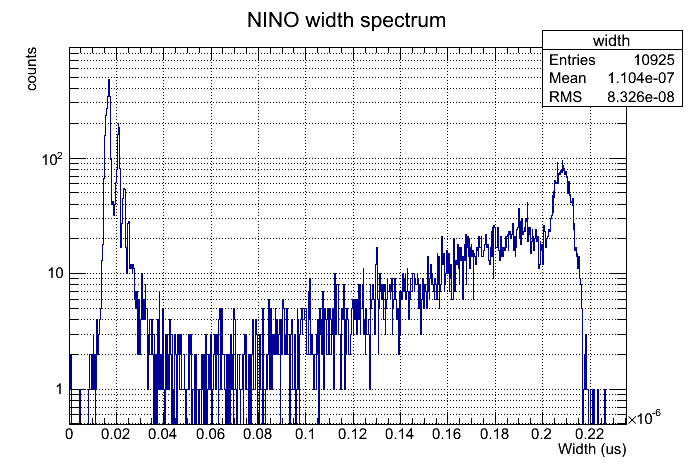
\includegraphics[width=9cm]{../Pictures/Chapter_8/spectrum_NINO.png}
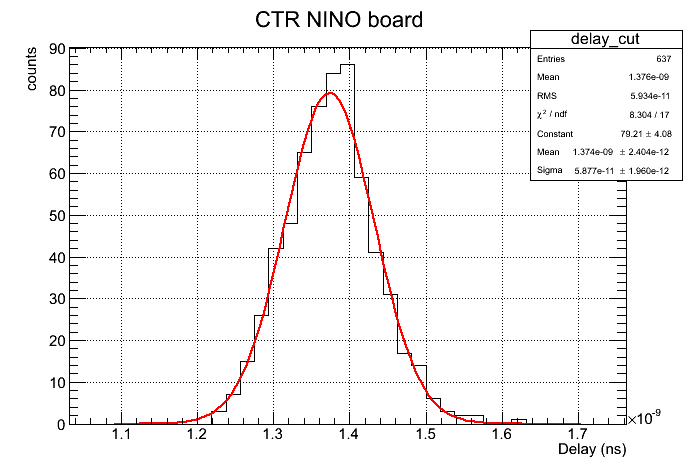
\includegraphics[width=9cm]{../Pictures/Chapter_8/CTR.png}
\end{center}
\caption[Start characteristics]{Example of start spectrum (top) and measured CTR at the photopeak (bottom).}
\label{fig:start}
\end{figure}

The electronics contribution depends on the data acquisition electronics and its noise level. This contribution can be estimated as
\begin{equation}
\sigma _{noise} = \frac{RMS _{noise}}{dV/dt}
\end{equation}
where the RMS of the noise is determined from the pedestal of the signal and $dV/dt$ is the slew rate. In this case it can be estimated at 37 ps (for a complete discussion see \cite{Gundacker2014}). 

\subsection{Characteristics of the stop signal}
The stop signal is a is a Hamamatsu R3809U-50 MCP-PMT. In order to estimate the contribution of the stop signal to the total IRF the MCP time response was measured with the aid of a high resolution laser.
The setup is composed by a Picosecond Diode Laser-Pilas head and a series of optical filters to reduce the light intensity hitting the photo detector down to less than one photon per excitation. The two signal are than routed to a LeCroy Oscilloscope LeCroy DDA 735Zi (10 GS/s) and data analysis is performed off line.
In order to measure the MCP SPTR a high resolution laser is needed, matching the wavelength of emission of the scintillator measured in TCSPC, if possible. The Pilas laser delivers a 28.9 ps pulse (FWHM) at a frequency of 100 kHz and a wavelength of 419 nm. The rising edge of the laser trigger is shown in figure \ref{fig:trigger}.
\begin{figure}[htbp]
\begin{center}
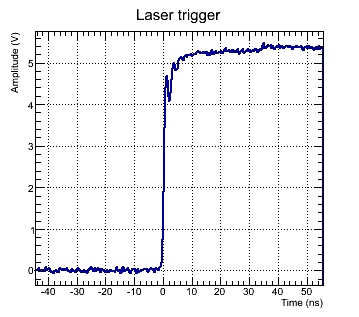
\includegraphics[width=8cm]{../Pictures/Chapter_8/laser_trigger.png}
\end{center}
\caption[Laser trigger]{Rising edge of the laser trigger.}
\label{fig:trigger}
\end{figure}
To extract the time difference between the laser trigger and the MCP signal, an offline analysis was performed. The digitized pulses were saved and analysed with the software package ROOT. A threshold for trigger was set at 5 mV on the MCP and the time difference was calculated in the interpolated signal. Therefore the sampling of the signal goes from 10 GS/s to 100 GS/s. 
\begin{figure}[htbp]
\begin{center}
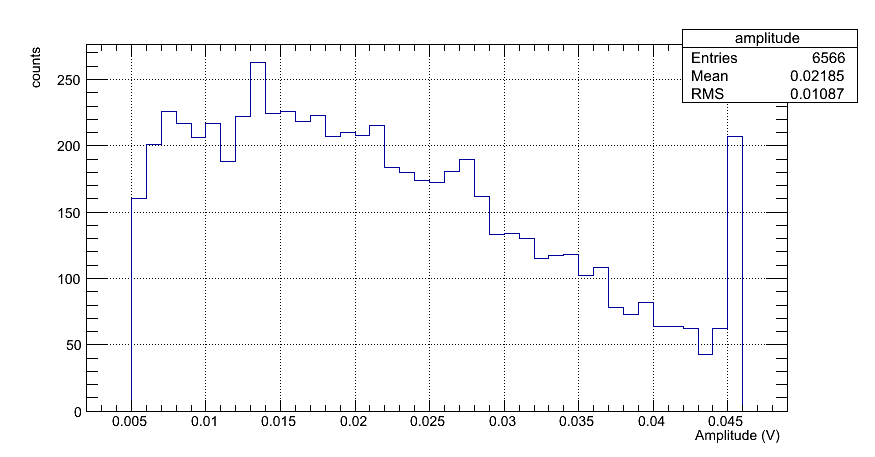
\includegraphics[width=9cm]{../Pictures/Chapter_8/amp_MCP.png}
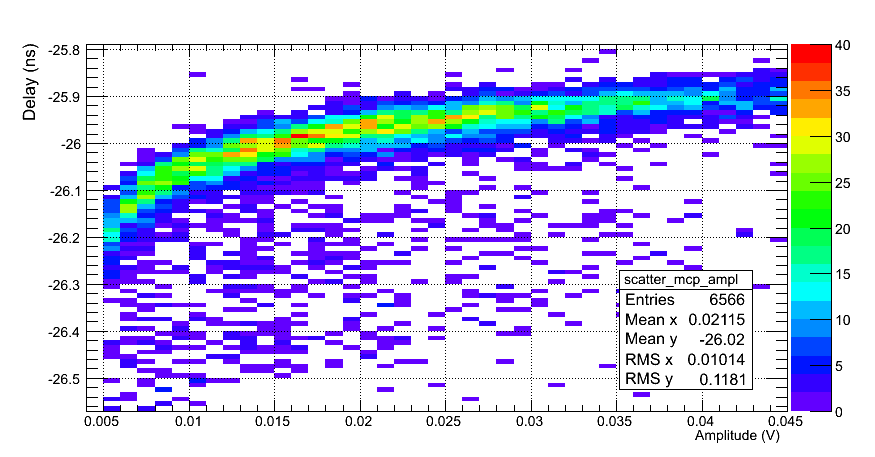
\includegraphics[width=12cm]{../Pictures/Chapter_8/time_walk_mcp.png}
\end{center}
\caption[Time walk of the MCP-PMT]{Amplitude spectrum for the MCP-PMT (top) and scatter plot amplitude - delay (bottom).}
\label{fig:mcp_laser}
\end{figure}
As shown in figure \ref{fig:mcp_laser}, the amplitude of the MCP varies considerably on the range considered, that is between 5 mV and 50 mV, where most of the signals lie. A saturation effect due to the limited amplitude window of the oscilloscope is also present, but removed with a cut in data analysis. This variation makes the stop detector prone to important time walk. 
The possibility of storing separately the digitized pulses allow for a complete selection and correction of these events. The scatter plot in figure \ref{fig:mcp_laser_walk} is corrected through a simple time walk correction.
If we define the real time stamp brought by the signal as t$_{real}$, the threshold crossing time t$_{measured}$ and the jitter given by the time walk we can write
\begin{equation}
t_{ideal} = t_{measured} - t_{walk}
\end{equation}
and we can extract the walk correction as
\begin{equation}
t_{walk} = A + B\cdot E^{C}
\end{equation}
where E is a measure of the charge collected. In this case it will be the amplitude of the MCP-PMT signal.
\begin{figure}[htbp]
\begin{center}
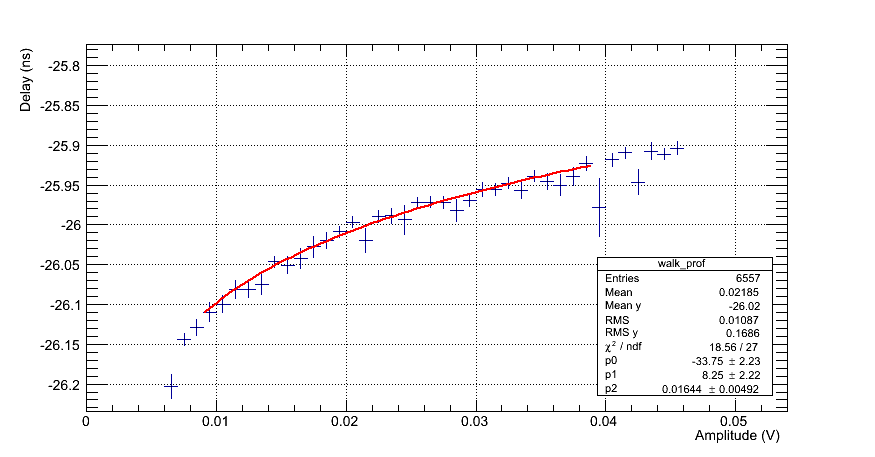
\includegraphics[width=12cm]{../Pictures/Chapter_8/time_walk_corr.png}
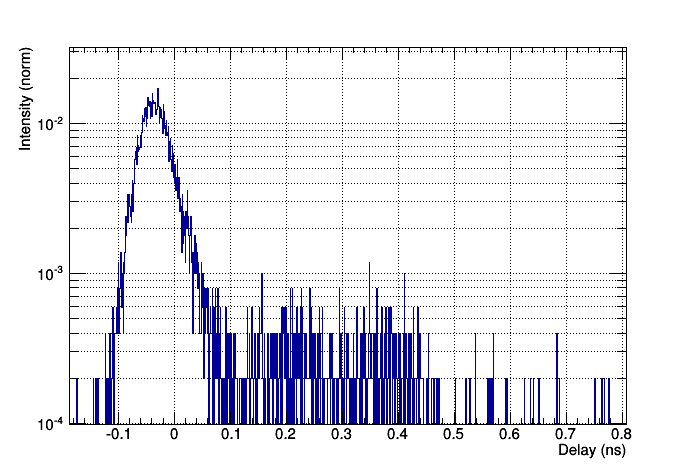
\includegraphics[width=9cm]{../Pictures/Chapter_8/laser.png}
\end{center}
\caption[MCP corrected response (laser trigger)]{Time walk correction on the spectrum profile, MCP-PMT against laser trigger (top) and resulting corrected response (bottom).}
\label{fig:mcp_laser_walk}
\end{figure}
At this point the spread on the time difference spectrum shown in figure \ref{fig:mcp_laser_walk} is given by four phenomena:
\begin{itemize}
\item width of the laser signal
\item jitter on the laser trigger
\item SPTR of the detector
\item electronics noise
\end{itemize}
It is natural to consider this processes uncorrelated so to concur to the smearing of the time distribution as
\begin{equation}
\sigma _{TOT}^{2} = \sigma _{SPTR}^{2} + \sigma _{laser}^{2} + \sigma _{trigger}^{2} + \sigma _{noise}^{2} 
\end{equation}
The laser width was taken from the data sheet, and amounts to 30 ps FWHM. The laser trigger can be substantially neglected as it amounts for $\sim$ 4 ps FWHM. Given the slew rate of the signal the $\sigma _{noise}$ amounts to $\sim$ 10 ps.

The spectrum measured can be grossly modelled as a Gaussian with a tail towards high delays. 
We notice from figure \ref{fig:mcp_laser} that ion feedback modifies the signal at higher times but it is almost two order of magnitude lower than the peak, as it is expected from a Chevron configuration. Considering the Gaussian peak we find $\sigma _{TOT} =$ 25 ps, so that we can infer    $\sigma _{SPTR} = $ 18 ps, given that $\sigma _{noise}^{2}$ amounts to 10 ps and $\sigma _{laser}^{2}$ to 13 ps.

\subsection{IRF measurements}
The last step is the measurement of the impulse response function (IRF), that is global variance on the estimate of the time stamps given by the combined effect of the start and stop uncertainties. This time spectrum needs to be deconvolved from the time spectrum of the sample measured in order to extract the parameters of the fluorescence.
In order to estimate the impulse response function, the set up presented in the previous section was used without the scintillation sample. The start signal retains the same characteristics, but the stop signal is given by a direct interaction in the MCP-PMT. This allows to disentangle the measured curve from the effect of the crystal, time constants and travel spread of the photons.
\begin{figure}[htbp]
\begin{center}
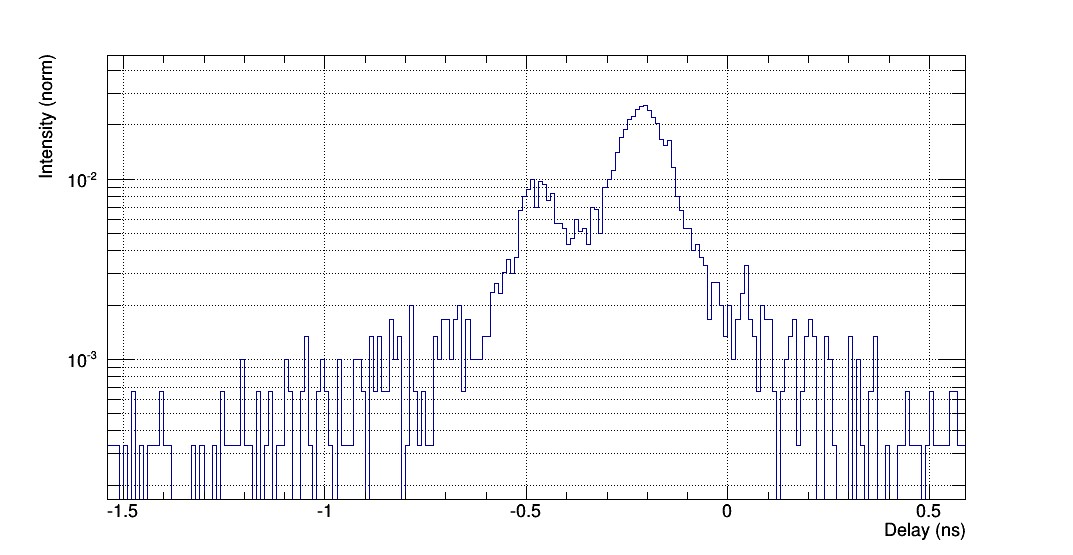
\includegraphics[width=9cm, heigth=6cm]{../Pictures/Chapter_8/response_cer_10}
\end{center}
\caption[Corrected IRF]{Measured response of the stop signal (MCP) against start signal (SiPM).}
\label{fig:ceren_10}
\end{figure}

The time walk corrected time spectrum is shown in figure \ref{fig:ceren_10}. Two separable components are present, separated by $\sim$ 300 ps.
In this configuration, The processes that concur to the time spectrum are:
\begin{itemize}
\item Cerenkov photons produced by $\gamma$ photons impinging in the entry window of the MCP-PMT
\item direct interaction of the $\gamma$ photons in the MCP stack
\end{itemize}
The delay of the two processes is contained in a time window of $\sim$ 300 ps.
Given the large variation in the output signal of the MCP it is not possible to select event by event with a pulse shape rejection method.
Using a simple Geant4 simulation it is possible to show that Cerenkov photons produced in the window need to interact in the photo cathode and then allow time for the produced photo electron to travel in the electric field to the MCP stack. In figure \ref{fig:drift} the times of Cerenkov production in the entry window and the time of a $\gamma$ photon interaction in a MCP stack is shown.
\begin{figure}[htbp]
\begin{center}
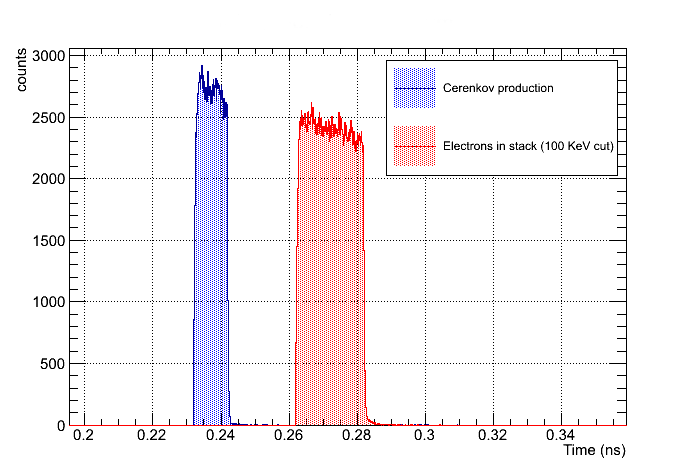
\includegraphics[width=9cm]{../Pictures/Chapter_8/interaction_time_spectrum.png}
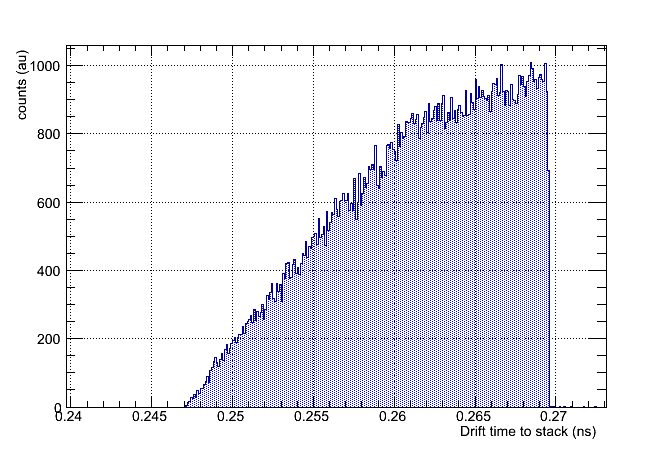
\includegraphics[width=9cm]{../Pictures/Chapter_8/drift_image_final.png}
\end{center}
\caption[Stack and Cerenkov simulation]{Time of interaction simulate for MCP stack and entry window Cerenkov photons (top) and drift time of electrons after the photo cathode (bottom). }
\label{fig:drift}
\end{figure}
It is then necessary to add the drifting time of the electrons between the photo cathode and the first MCP stack, based on the geometry of the detector. The drifting electric field by design is given by the voltage divider of the detector, and amounts to 310 kV/m.
As shown on the right side of figure \ref{fig:drift} the drifting time of the electrons matches the time difference in the two components present in the measured IRF, and small deviations can be ascribed to partial knowledge of the detector materials and geometry of the electric field in the drifting region.

This phenomenon can be experimentally shown by suppress one of the two processes. The setup was then slightly changed by tilting the MCP-PMT with respect to the start-source system.
\begin{figure}[htbp]
\begin{center}
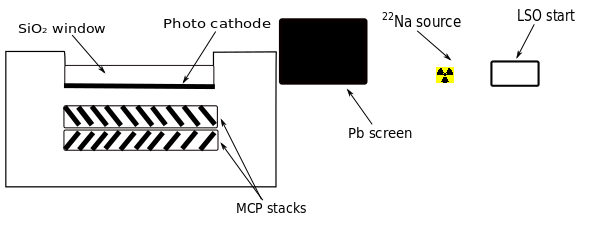
\includegraphics[width=9cm]{../Pictures/Chapter_8/screen_irf_2.png}
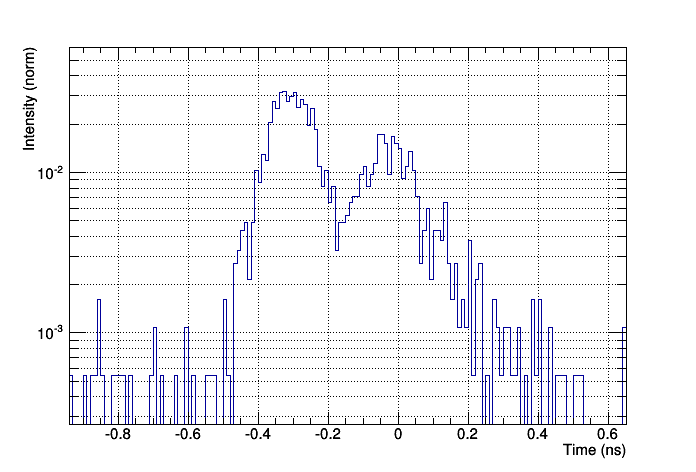
\includegraphics[width=12cm]{../Pictures/Chapter_8/turn_1.png}
\end{center}
\caption[Setup for $\gamma$ interaction in stack]{Setup for $\gamma$ interaction in stack (top) and spectrum recorded (bottom)}
\label{fig:twist2}
\end{figure}
\begin{figure}[htbp]
\begin{center}
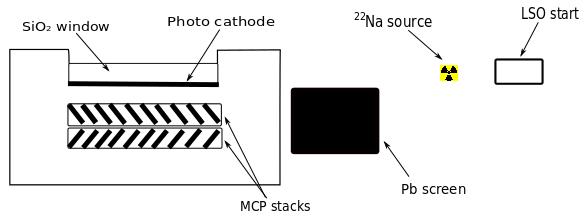
\includegraphics[width=9cm]{../Pictures/Chapter_8/screen_irf.png}
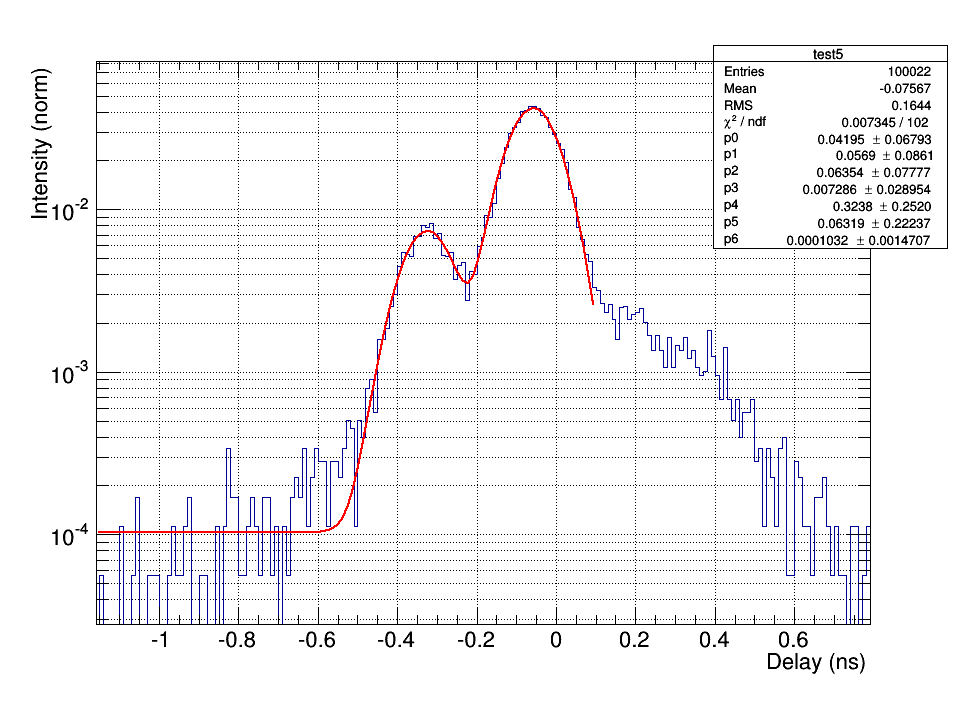
\includegraphics[width=12cm]{../Pictures/Chapter_8/turn_2.png}
\end{center}
\caption[Setup for Cerenkov production in the window]{Setup for Cerenkov production in window (top) and spectrum recorded (bottom)}
\label{fig:twist1}
\end{figure}
Then a lead screen was placed in between and two set of measurements was performed, as shown in figure \ref{fig:twist1} and \ref{fig:twist2}:
\begin{itemize}
\item a first one with the screen covering the direct line of interaction between the source and the position of the MCP stack deduced from the design of the detector
\item a second one with the screen covering the section of the entry window
\end{itemize}
It was then possible to suppress, respectively, the direct $\gamma$ interaction in the stack and the Cerenkov production in the window. The relative intensity of the two peaks is reversed, as shown in figure \ref{fig:twist2}. 
The final time resolution can be inferred from the 
last figure, since the IRF to be deconvolved is composed only by the part of the spectrum related to photo electrons. As will be explained below, the direct interaction of $\gamma$ photons in the stack brings additional spurious background to the spectrum, but it is not related to the scintillation pulse. Nevertheless the two peaks show similar width, and this is due to the fact that the resolution is dominated by the start signal, which is far worse and the slight difference given by the electron drift is negligible.
As a consequence, we cut on the Cerenkov part of the IRF spectrum, and extract the width as a $\sigma _{IRF}$ = 73 ps. This is in substantial agreement with the discussion of the previous section since $\sigma _{IRF}^{2} = \sigma _{stop}^{2} + \sigma _{start}^{2} + \sigma _{noise}^{2}$, where $\sigma _{start}$ = 62 ps, $\sigma _{noise}$ = 37 ps and $\sigma _{stop}$ = 18 ps.

\subsection{Control of the bias fraction}
The main advantage of using the available oscilloscope as a digitizer of the pulses for off line analysis is the possibility of extracting multi time stamps. This allows for a multi-hit TDC approach. 
Thanks to the fact that signals from MCP-PMT are very fast, i.e. completely contained in 1 ns, the dead time is very low and so it is the biased fraction of events. 
Starting from the considerations previously stated in chapter 6, it is possible to control this fraction by counting the number of pulses per event.
Usually the biased fraction is qualitatively controlled by calculating the geometric factor of the setup and by keeping the number of counts well below one per start signal. This was also the approach used in the case of VUV measurement, where  no multi hit TDC was available.
In the case of the $\gamma$ setup, also given the low number of counts and the difficulties in collecting a high statistics, it is necessary to keep the rate as high as possible, while still being sure not to introduce significant bias in the measurement.
In this setup it is possible to control in real time the number of pulses per event that should follow a Poisson distribution, as shown in figure \ref{fig:twist1} for a LSO:Ce, Ca crystal. The extraction of the average allows to completely control the bias fraction, and this was done for all the samples measured.
\begin{figure}
\begin{center}
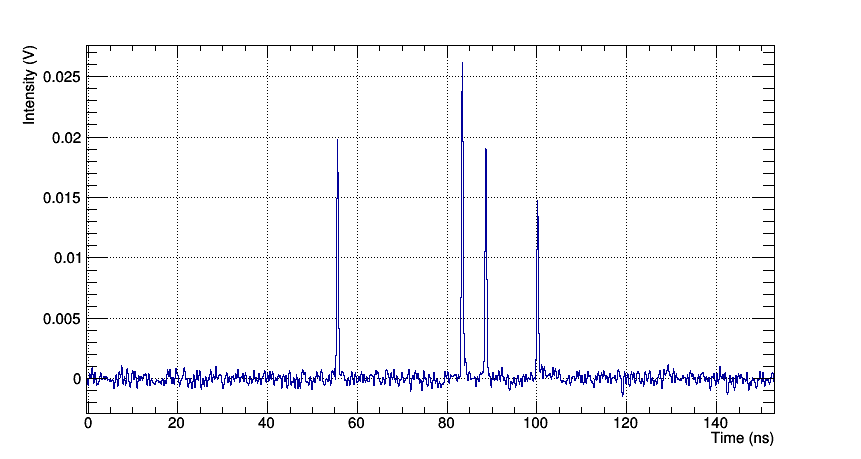
\includegraphics[width=9cm]{../Pictures/Chapter_8/multi.png}
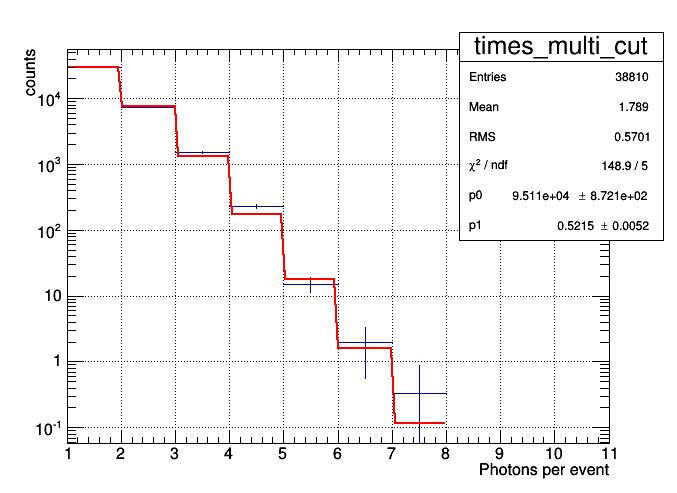
\includegraphics[width=9cm]{../Pictures/Chapter_8/multi_pois.png}
\end{center}
\caption[Multi hits in $\gamma$ setup]{Example of multi hit event (top) and distribution of pulses over the events (bottom).}
\label{fig:twist1}
\end{figure}
\subsection{Background}
In the measurement campaign conducted two separate background processes intervene:
\begin{itemize}
\item random coincidences
\item direct interaction of a $\gamma$ in the detector
\end{itemize}
For what concerns random coincidences they should be kept at a low level, in order not to worsen the uncertainty on the parameter extraction at the fit level. Indeed the important parameter is the signal to noise ratio and this aspect depends strongly on the light yield of the crystal measured, and on the geometry of the system. Nevertheless this kind of event is taken into account in the fit procedure, and in principle the only disadvantage is the necessity for higher statistics to be collected.

The direct interaction of a $\gamma$ in the detector, on the other hand, could severely bias the measurement, in the time window where the rising edge of the crystal lies. 
The active area of the MCP is quite large, given the size of the entry window, with a diameter of 11 mm. This makes direct interaction in the detector quite likely.
This is easily taken into account in the case of 511 keV $\gamma$, since they are emitted back to back. In this case it is sufficient to tilt the stop detector with respect to the sample to measure, with an angle of 90 $^{\circ}$C.

As previously explained, in addition to the 511 keV $\gamma$ photons produced by the annihilation of the positron, the $^{22}$Na de-excite to the $^{22}$ Ne ground level by emitting a 1.274 MeV $\gamma$. 
The de-excitation $\gamma$ is emitted isotropically and can interact in the detector after a gate is open on the start arm, unrelated to any scintillation event in the sample.
As shown in \ref{fig:twist2} this events happen exactly on the rise time of the signal, since the delay introduced by the geometry is negligible.
It is not possible to select on a pulse shape basis since the MCP amplitude largely varies, and there is no separable difference between signals coming from a 1.274 MeV event and a photo electron event.

Thus in order to restrict the influence of this events, which become less and less problematic as light yield of the sample measured increase, two approaches are possible:
\begin{itemize}
\item screen the detector from the source
\item optically delay the scintillation light in order to easily cut spurious events from direct interaction.
\end{itemize}
The first solution was chosen for time constraints, but the optical delay will be implemented in the future. In particular 5 cm of lead blocks were positioned in between, that allow to stop 95$\%$ of the incoming $\gamma$ photons (density and stopping power taken from \cite{nist2005}). The setup is shown in figure \ref{fig:twist3}.
%\begin{figure}
%\begin{center}
%\includegraphics[width=7cm]{../Pictures/Chapter_8/.png}
%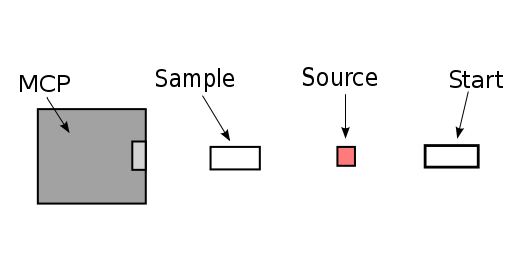
\includegraphics[width=7cm]{../Pictures/Chapter_8/setup_direct.png}
%\end{center}
%\caption[Background biased measurement]{Highly biased time profile of CeF$_{3}$ sample (top) and relative setup (bottom).}
%\label{fig:twist2}
%\end{figure}
\begin{figure}
\begin{center}
%\includegraphics[width=7cm]{../Pictures/Chapter_8/.png}
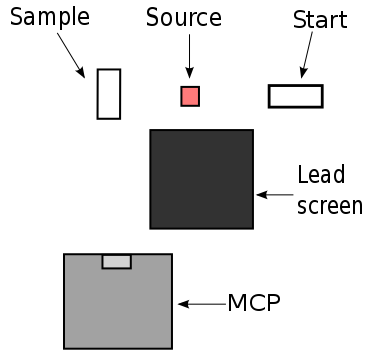
\includegraphics[width=5.5cm]{../Pictures/Chapter_8/setup_twist.png}
\end{center}
\caption[Background suppressed setup]{Final setup for measurement. The Lead block provides screening against direct excitation.}
\label{fig:twist3}
\end{figure}

\section{Data analysis}
Due to time constraints not all the samples measured in VUV could be measured with the $\gamma$ setup, though the proof of concept was delivered for future completion of the study.
The samples measured in the $\gamma$ setup were
\begin{itemize}
\item LYSO:Ce (Proteus)
\item LGSO:Ce
\item LSO:Ce (CTI)
\item CeF$_{3}$
\item LSO:Ce,Ca (Agile)
\item LuAG:Ce (0.13$\%$)
\item BGO
\end{itemize}
The data extracted were analyzed offline for cuts and time walk correction. 
The rise time parameter was extracted with the iterative re convolution algorithm presented in chapter 6, and the error was evaluated as likelihood confidence interval on the $\Delta$L.

\subsection{Cuts and background estimation}
The IRF measurement was performed at the beginning of the measurement campaign and repeated at regular intervals to correct for eventual drifts, but no significant drift was observed.
On the data collected for off line analysis the first cut performed is the photo peak selection on the start signal, that for the NINO signal happens between 200 and 220 ns, at the 511 keV peak of the $^{22}$Na.

For the MCP data two set of manipulations were performed: on the amplitude of the MCP to avoid saturation effect and for time walk correction. 
The MCP signal was cut between 10 and 40 mV, which is the interval that contains the 70$\%$ of the pulses collected. At this point the signal was corrected for time walk.

As previously explained, the background can play an important role in the measurement, especially in the case of crystals with low or very low light yield, which is the case of CeF$_{3}$ for example. 
In order to control this a lead screen was positioned between the source and the MCP to suppress the count rate from direct interaction in the stack. Additionally a quick background measurement was performed, to ensure that the background count rate could be neglected.

\subsection{Fit procedure}
The fit procedure has been presented in chapter 6 and it consists in the minimization of the function $-\log{L}$, where the likelihood function $L$ is given by the convolution of the model and the IRF.
The function used for the fit is a simple multi-exponential model for n decay component as
\begin{equation}
p(t) = \sum _{i = 1}^{n} \frac{P_{i}}{\tau _{d, i} - \tau _{r, i}}\left( e^{-\frac{t-t_{shift}}{\tau _{d}}} - e^{-\frac{t-t_{shift}}{\tau _{r}}} \right) + C_{bg}
\end{equation}
where $\tau _{shift}$ is the turn-on of the scintillation pulse and $C_{bg}$ is the background level.
Two factors contribute to worsen the confidence and accuracy of the measurement: the already quoted background problem and the low statistics accumulated.
Indeed due to time constraints it was not possible to collect the statistics necessary to restrict the confidence level to the level of the VUV measurement. Given the discussion in chapter 6, and considering figure \ref{fig:likelihood} on page \pageref{fig:likelihood}, the confidence level doubles for less than 500000 counts and a small bias towards faster rise times is introduced, due to the weight on the first part of the pulse.

For what concerns the range influence, similar observations can be made with respect to the VUV setup, and we will consider the optimal range over bin 15000.
\section{Results}
\subsection{Data}
The LYSO:Ce (Proteus), LYSO:Ce (Sipat), LS0:Ce (CTI) and LGSO:Ce samples were measured in two configuration: naked and Teflon wrapped. 
The CeF$_{3}$, LuAG:Ce, BGO and LSO:Ca,Ce (Agile) samples could not be measured in naked configuration. The light collected is too low to guarantee compatible accumulation times. This is partly given by the low light yield of the samples, as shown in chapter 5, and the low quantum efficiency for the emission spectra of the samples.
The results are shown in \ref{table:table_gamma} and examples of plots for the crystal measured are reported along with the likelihood residuals.

\begin{figure}[htbp]
\begin{center}
\includegraphics[width=9cm]{../Pictures/Chapter_8/2737.png}
\includegraphics[width=9cm]{../Pictures/Chapter_8/2737_wrapped.png}
\end{center}
\caption[LYSO Sipat and Proteus profile]{Fit data and likelihood residuals for LYSO Proteus naked (top) and LYSO Proteus Teflon wrapped (bottom).}
\label{fig:wnw_proteus}
\end{figure}

\begin{table}[h]
\begin{center}
\begin{tabular}{|l|l|l|l|}
\hline
Crystal  & $\tau _{r}$ naked & $\tau _{r} wrapped$ \\
\hline
LYSO Sipat & 85$_{-40}^{+38}$ ps & 160$_{-43}^{+34}$ ps \\
\hline
LYSO Proteus & 73$_{-38}^{+33}$ ps & 145$_{-34}^{+32}$ ps \\ 
\hline
LSO CTI & 90$_{-45}^{+40}$ ps & 138$_{-46}^{+34}$ ps \\ 
\hline
LGSO & 84$_{-43}^{38}$ ps & 146$_{-37}^{+35}$ ps \\  
\hline
LSO:Ca &  & 124$_{-35}^{+33}$ ps \\ 
\hline
CeF$_{3}$ &  & 145$_{-51}^{+43}$ ps  \\
\hline
BGO & & 153$_{-46}^{+33}$ ps \\
\hline
LuAG & & $380_{-40}^{+35}$ ps \\
\hline
\end{tabular}
\end{center}
\caption[Rise time values for $\gamma$ bench]{Values of rise time measured for naked and Teflon wrapped crystals}
\label{table:table_gamma}
\end{table}

\subsection{Discussion}
In order to compare the results with the data obtained in chapter 7, it is necessary to compare the values guided by a simulation study.
As already discussed, we should generically consider three steps: the ionization phase down to the thermalization stage, the relaxation itself and the transportation of the optical photons produced.
In the case of VUV excitation only the first two steps were investigated. Due to the geometry of the experiment no volume effect occurred. 
In the setup presented in this chapter, on the other hand, the excitation happens inside the crystal volume and thus photon transportation introduce a non negligible effect.
Moreover, at 511 keV the electrons produced via photo electric effect are above Cerenkov threshold and thus they can produce Cerenkov photons.
The large error on the measurement weakens the analysis which is not completely conclusive, but it is already interesting to compare the data collected.

All the samples could be measured with Teflon wrapping, since it increases the probability of a photon to be coupled out.
The data collected confirms the observations derived from the VUV analysis. LSO and similar Cerium doped compounds showed faster decay times with respect to the Garnet sample measured.
In this case the values extracted are significantly higher than the respective counter part in VUV excitation.
This is given by two aspects: the Cerenkov production and the transportation inside the volume. This is been diffusively explained in chapter 6 with a simulation study.
In our case, that is samples of 2x2x3 mm$^{3}$ and 2x2x5 mm$^{3}$ geometry brings about 10 ps at the extraction to the intrinsic rise time.
For what concerns Cerenkov photons there is in principle a difference that depends on the properties of the samples measured. In order to assess this difference it would be necessary to measure crystals of different material, but same size with high statistics. This was not possible, but for the case of LSO/LYSO samples measured we can conclude that Cerenkov photons bring additional 10 to 20 ps to the extracted rise time with respect to the intrinsic one.
It has been already underlined that energy deposition above the ionization threshold happens on shorter time scales, thus we do not attribute any difference in the rise time extracted to ionization. Therefore we can attribute the rise time measured in VUV to thermalization processes, and this will be added to the other processes contributing to rise times in $\gamma$ excitation.
This is the case for the crystals measured in naked condition (LSO, LYSO, LGSO): with respect to VUV measurement they all show slower rise times, from $\sim$30 ps to $\sim$80 ps as can be easily inferred from the comparison of the data tables.
It should be noted that due to the low statistics and the consequent relevant error on the measurement ($\sim$ 50 ps for every sample) it is not statistically relevant to extend the analysis to possible comparison between different crystals of the same groups (e.g. LSO and LGSO).

A second important observation is given by the measurement of samples with Teflon wrapping.
The considerations of chapter 6 allow to conclude, on a  simulation base, that a diffusive wrapping modelled on the optical characteristics of Teflon, should increase the photon extraction efficiency of the system. By doing this, the useful angle for extraction is enlarged, and photons that underwent multiple bounces may be extracted. This entails a gain in the light yield, but a sensible increase in the time RMS. This in exchange leads to higher rise times.
This is reflected in the measurement of the samples. We measured all the samples with Teflon wrapping and the values obtained are compatible with the simulation study. Indeed values for Teflon wrapped crystal may go as high as 150 ps.

\subsection{Limitations and perspectives}
The feasibility of the rise time measurement has been proved with a table top setup. The quantity accessible is an effective rise time that takes into account relaxation of the excited states of the lattice as well as the production of Cerenkov photons and the optical transportation of light to the detector.

A future objective is to measure the low light yield crystals in naked conditions, so to completely characterize the set of samples. With respect to this, the main limitations of the setup already outlined are the resolution of the start signal, the count rate and the background from direct interaction in the MCP stack, and they influence both the trueness and precision of the measurement.

The start signal is the main limiting factor in terms of resolution achievable. Indeed the IRF suffers mainly from the limited resolution given by the tagging and the SiPM at $\sim$ 60 ps, the other contributions being well below this value. Unfortunately this limit is not trivial to overcome, for a measurement in radioluminescence. 
In particular, as shown in chapter 6, transportation of optical photons and surface state or wrapping take a relevant part of the measured rise time. This means that even without volume excitation it is necessary to work on the geometry of the system in order to study this contribution.
VUV excitation setups do not give the necessary flexibility for such a study; an alternative could be given by table top x-ray pulsed machines, see for example \cite{Derenzo2000}.

For what concerns the count rate, long accumulation times entail a duration for measurement of several days. In order to safely screen the detector from the direct interaction of $\gamma$ photons the geometric efficiency of the system is lowered and so the count rate.
A solution to this problem is to optically delay the scintillation light in order to easily cut spurious events from direct interaction. Moreover a different detection method could in principle avoid this contribution, based for example on Geiger mode APD cells or a streak camera.